%%% File: ./inputs/parts/COMPILING_PROGRAMS.tex

%%%%%%%%%%%%%%%%%%%%%%%%%%%% BEGIN COMPILING PROGRAMS %%%%%%%%%%%%%%%%%%%%%%%%%%%

%%% \subsection*{Embodied Cognition}

%%% \subsection*{Conscious Attention}

%%% \subsection*{Action Selection}

%%% \subsection*{Executive Control}

%%%%%%%%%%%%%%%%%%%%%%%%%%%% BEGIN DECEMBER 29 NOTES %%%%%%%%%%%%%%%%%%%%%%%%%%%%

\subsection*{Compiling Programs}

%%% START A 

The activity in the system comprised of the basal ganglia, cerebellum and motor cortex plus the brain stem and spinal cord is perhaps the closest the mammalian brain comes to writing and executing programs. Generally referred to as "motor programs", they control all of your voluntary movements and, in humans, they play an important role in language.

The right panel in Figure~{\urlh{#fig_White_Matter_Tracts_Long_Distance}{\ref{fig_tracts}}} shows the white matter reciprocal connections between the frontal cortex and the cerebellum that are believed to facilitate higher-order cognitive functions. Curiously, it is possible to lead a relatively normal life even if you were born without a cerebellum, difficulty speaking and walking being the most obvious deficits.

The distribution of cell types and neural circuitry of the cerebellum is reminiscent of the hippocampal formation and there are several detailed models of the cerebellum~\cite{MarrJoP-69,AlbusMB-71,ItoCEREBELLAR-CORTEX-18} that have inspired useful machine learning techniques~\cite{Albus75}, and yet discoveries in the last decade have challenged prevailing opinions.

It was believed that all communication between the basal ganglia and cerebellum was indirectly enabled via the cerebral cortex, but evidence now supports the existence of subcortical connections between the two suggesting that the basal ganglia, the cerebellum and the cerebral cortex form an integrated network~\cite{BostanandStrickNATURE-REVIEWS-NEUROSCIENCE-18}.

These new discoveries will likely have important ramifications for our understanding of these critical systems that will lead to new algorithmic insights that parallel those fueled by our study of the hippocampal formation Box~\colorred{D}. Here we focus on what the basal ganglia, the cerebellum and the cerebral cortex tell us about creating, selecting and coordinating motor programs.

%%% %%%%%%%%%%%%%%%%%%%%%%%%%%%%%%%%%%%%%%%%%%%%%%%%%%%%%%%%%%%%%%%%%%%%%%%%%%%%

The brain derives much of its utility from exploiting distributed representations and parallel processing. Even so, in big brains it is often useful bring representations from distant parts of the brain together and necessary to perform some computations serially with the results from one computation feeding into another. The human brain has evolved machinery that makes it possible for us to do both by making better use of existing memory systems and adapting circuits optimized for movement to communicate, plan and perform abstract reasoning.

The human brain makes extensive use of topographically organized representations, often contructing multiple maps with same topographic organization that can be aligned with one another to construct more abstract representation that retain the locality relationships of their constituent maps~\cite{WandelletalNEURON-07,WandelletalPTRS-B-05}. This is a subtle point and a generally underappreciated fact about organisms with a central nervous system responsible for coordinating behavior distributed across their peripheral nervous system. 

Several of the subcortical circuits we've discussed including the basal ganglia and hippocampus have access to sensorimotor areas of the cerebral cortex by way of the thalamus and the striatum, the latter being part of the basal ganglia. The thalamus consists of a set of nuclei that map specific subcortical inputs to the cortex and receive feedback from the same cortical areas. The striatum assists in coordinating cognitive functions, including both motor and action planning.

\begin{center}
  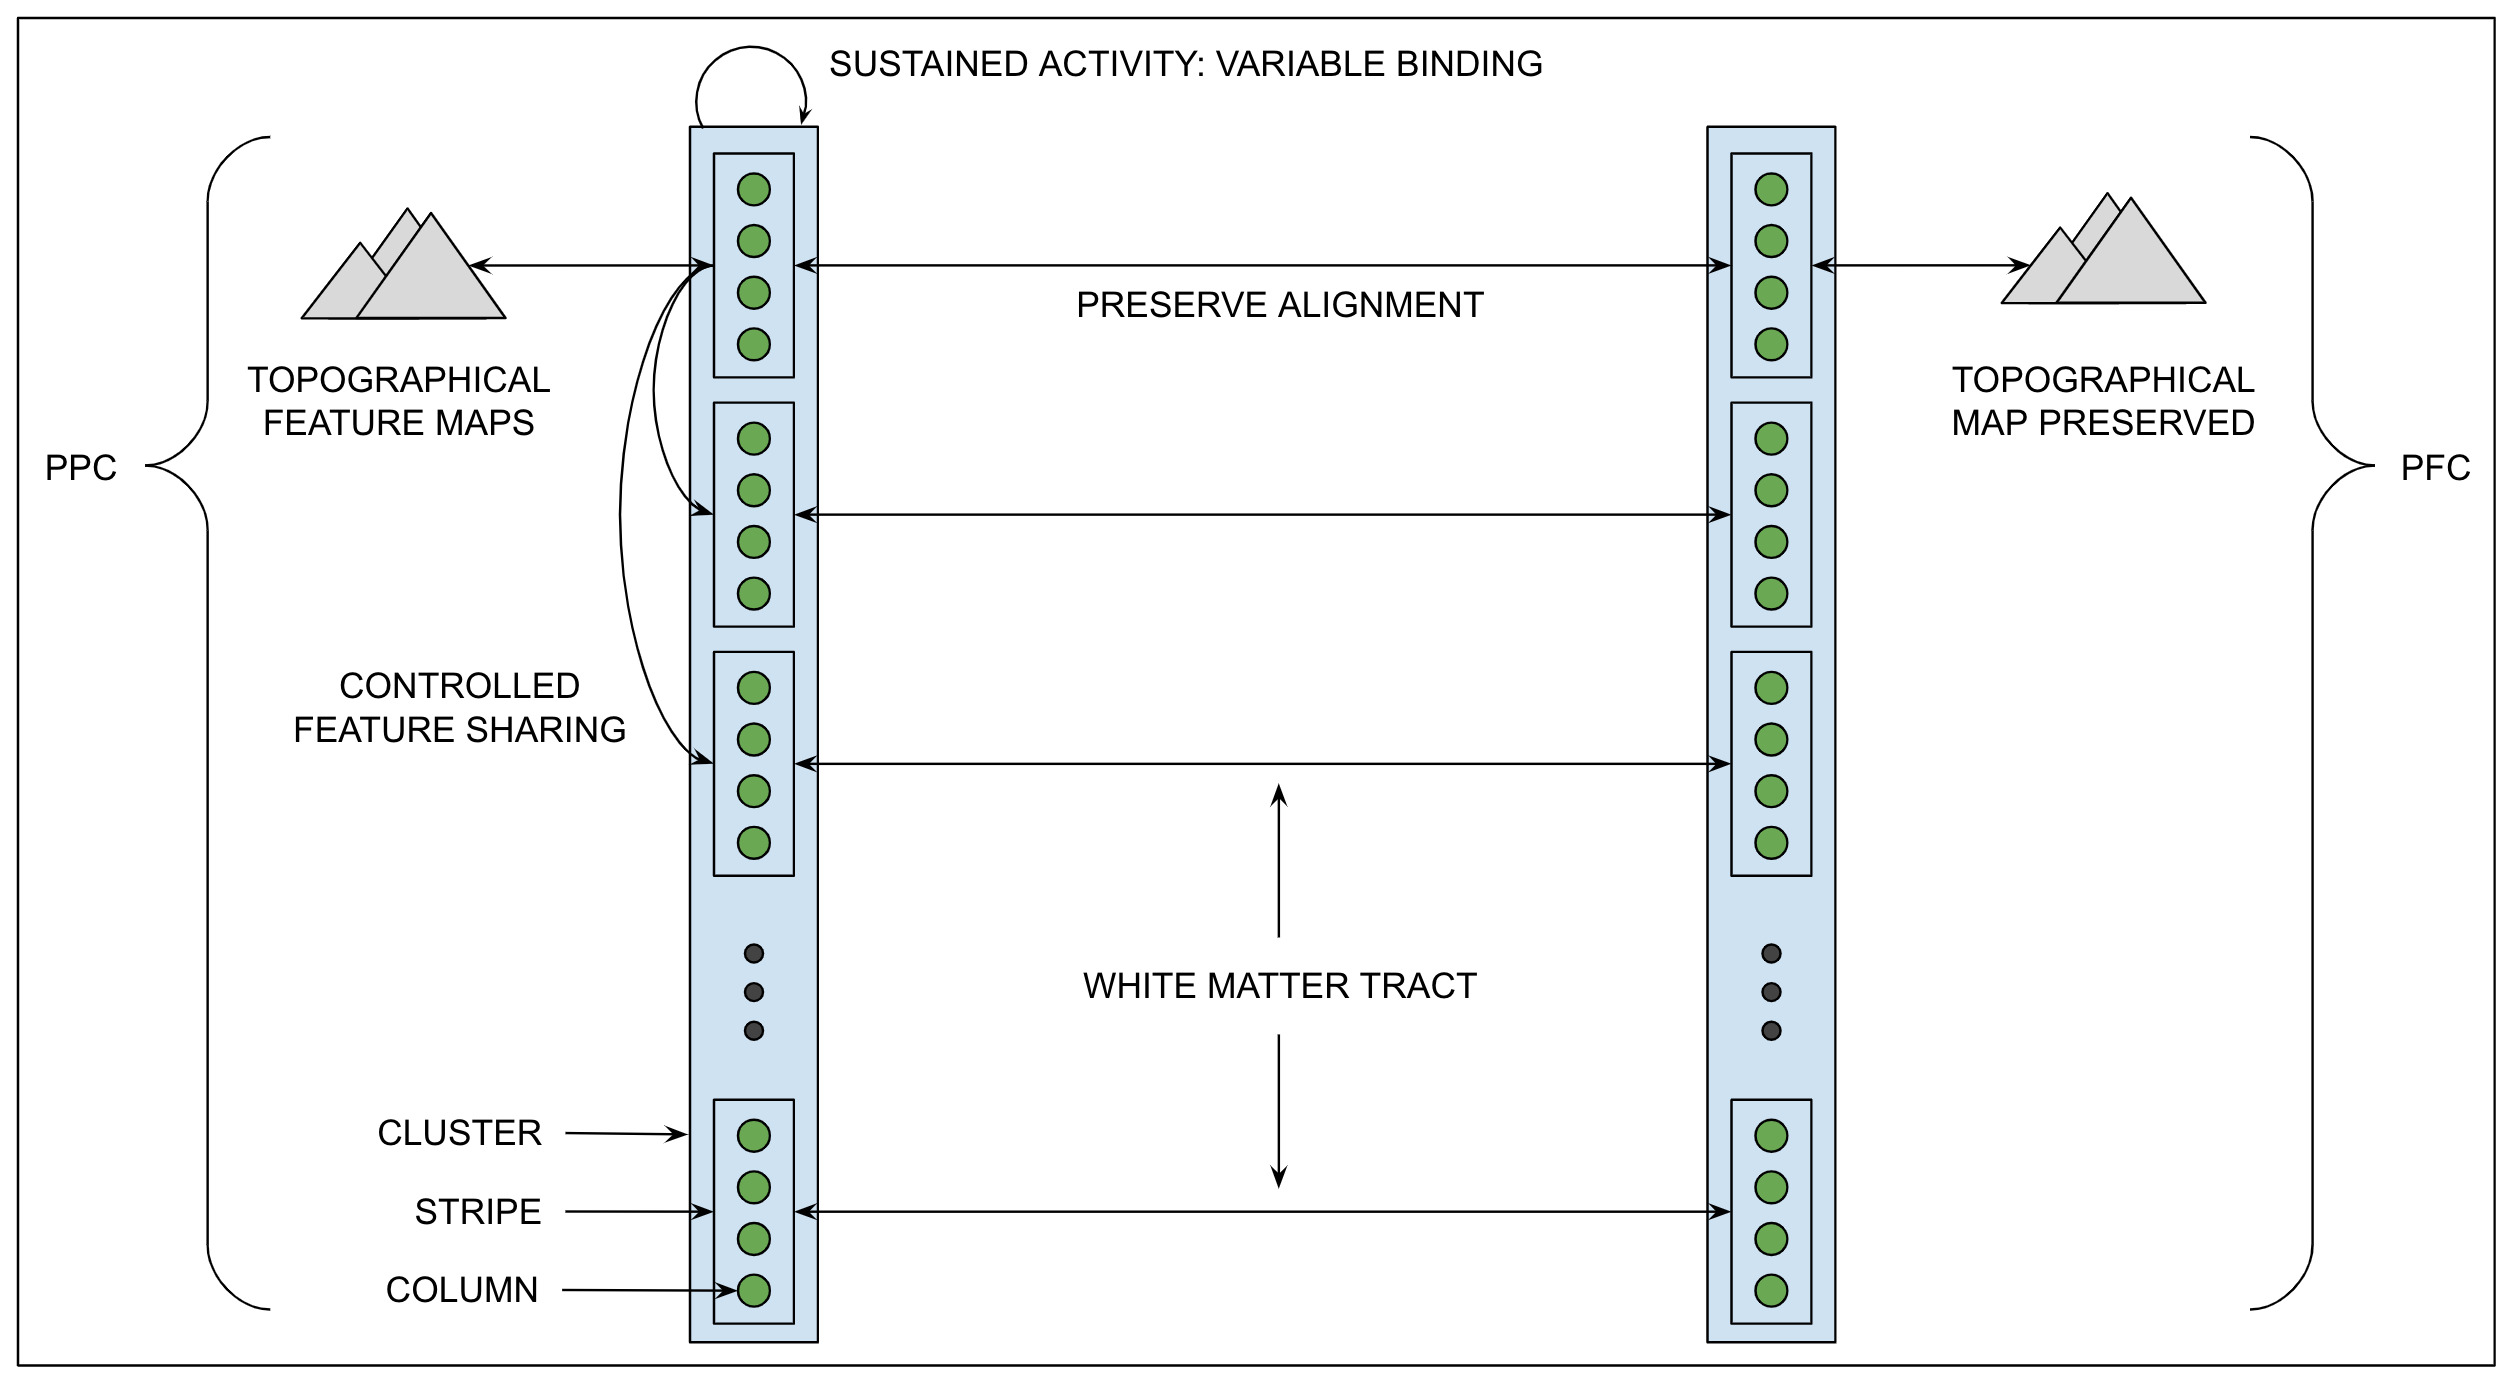
\includegraphics[width=800pt]{./figures/Columns_Stripes_Clusters_Topographic_Maps.png}
\end{center}

Much of the information moving around in the cortex is structured in the form of maps that align with the topography of the sensory and motor systems of the body, retinotopy of the visual cortex being one example. The striatum's distinctive striated appearance is due to its arrangement of specialized circuits called {\it{stripes}} that enable the basal ganglia to select and transfer information to distant locations in the cortex that have similarly striated and functioning circuits, preserving essential topographical features in the process~\cite{BarbasandGarcia-CabezasCOiN-16,LewisetalJNC-02}.

Each stripe is composed of columnar-shaped circuits called {\it{minicolumns}} that encode patterns of coordinated activity originating elsewhere in the cortex so it can brought together in one place for processing. Each stripe can be updated independently allowing the basal ganglia a great deal of discretion in creating a context for initiating subsequent computations at remote locations in the frontal cortex. These patterns of activity can be stored indefinitely providing a working memory system that supports a simple yet powerful method for binding variables and composing their values~\cite{OReillyetalCCN-12}.

Stripes are grouped in {\it{clusters}} that can reinforce or inhibit one another and clusters map to other clusters often by way of white-matter tracts that connect distant sensory and motor areas. Information is transferred preserving its topographic structure so processed information resulting from motion planning or other cognitive functions can be mapped back to its origin to support learning or stimulate muscle activity.

The activity in stripe clusters can be maintained or updated individually allowing for sustained or iterative processing and providing the basis for working memory. Information in multiple clusters can be combined to support a simple form of variable binding. The basal ganglia and prefrontal cortex can influence what information is transferred but the preserved alignment of the stripes within clusters dictates the origin of the information.

%%% STOP A 

%%%%%%%%%%%%%%%%%%%%%%%%%%%%% END DECEMBER 29 NOTES %%%%%%%%%%%%%%%%%%%%%%%%%%%%%

%%% START B

As we look more carefully at action selection and motion planning, it will help if we adopt standard terminology as it will both simplify our discussions and reveal aspects of the problem that we've neglected to take into account. In classical mechanics and robot motion planning, the parameters that define the configuration of a system are called {\it{generalized coordinates}} or {\it{degrees of freedom}}, and the vector space defined by these coordinates is called the {\urlh{https://en.wikipedia.org/wiki/Configuration_space_(physics)}{{\it{configuration space}}}} of the physical system. The following graphic shows a simple configuration space and two coordinate vectors referred to as configurations and illustrated here as two poses of a cartoon robot.

%%% %%%%%%%%%%%%%%%%%%%%%%%%%%%%%%%%%%%%%%%%%%%%%%%%%%%%%%%%%%%%%%%%%%% 

\begin{center}
  \includegraphics[width=250pt]{./figures/Two_Nearby_Points_in_Configuration_Space.png}
\end{center}

%%% %%%%%%%%%%%%%%%%%%%%%%%%%%%%%%%%%%%%%%%%%%%%%%%%%%%%%%%%%%%%%%%%%%%

\hrule{}

%%% %%%%%%%%%%%%%%%%%%%%%%%%%%%%%%%%%%%%%%%%%%%%%%%%%%%%%%%%%%%%%%%%%%% 

In the case of a robot, its actuators are restricted mechanically just as our movements are restricted by our skeletal structure and musculature. In robot planning, movement is further restricted by the obstacles in the robot's environment. These constraints limit the reachable space, corresponding to a lower-dimensional manifold called the {\it{configuration manifold}}. If you took a course from Jean-Claude Latombe or Oussama Khatib, you might remember that the complexity of path planning {\emdash{}} finding an uninterrupted path from one point to another in a given configuration space {\emdash{}} is worst-case exponential in the number of degrees of freedom.

That said, there are many efficient approximations~\cite{Latombe90} including Khatib's~\cite{KhatibIJRR-86} {\urlh{https://en.wikipedia.org/wiki/Motion_planning#Artificial_potential_fields}{{\it{artificial potential field}}}} method for escaping local minima and Kavraki and Latombe's~\cite{KavrakiandLatombeIEEE-94} method for randomized preprocessing of the configuration space. The former lends itself to artificial neural network implementations and the latter suggests that simple local search methods often suffice for many practical problems assuming sensory systems and servomechanisms able to exploit structural and environmental affordances.

The following is a narrative sketch of the mechanisms and related representations that guide the selection of motor plans. So far our characterization of robot motion planning is impoverished as an agent's representation of its internal state in that it leaves out the critical role of perception and feedback. Robust motion plans must necessarily include perceptual activities whose purpose it is to help guide movement, avoid obstacles including one's own body parts and facilitate accurate positioning and grasping.      

Configuration space is a kinematic model plus a static representation of the physical environment. This is not the same as {\it{phase space}} which emphasizes the system dynamics and includes the velocity and mass (momentum) of every particle. To serve as a basis for motion planning, an internal representation must capture not only the physical constraints that the body and environment impose on movement, but also the cognitive state of the agent incorporating current estimates of the location and velocity of nearby objects and body parts relative to the body's frame of reference and relevant knowledge about their properties and role in the agent's objectives.

There is a consensus that motor plans are represented in the primary, premotor and supplementary motor cortex in the frontal cortex adjacent to the central sulcus. The nearby somatosensory and proprioceptive association areas of the anterior parietal cortex are likely to figure prominently in planning movement, as are the sensory association areas in the posterior parietal cortex and in particular the dorsal visual stream also known as the "where" or "how" stream. These sources of relevant neural activity provide a rich context for action selection available directly to the basal ganglia to shape in the form of proposals or {\it{intentions}}.

We know that regions of the motor cortex are topographically mapped; in much the same way that nearby points in configuration space {\emdash{}} or at least on the corresponding low-dimensional manifold {\emdash{}} are joined by smooth trajectories through joint space. In lieu of an internal representation for abstract goals and the neural circuits required to act upon them, we borrow the term {\it{setpoint}} from control theory to denote the target state of the controlled system. Negative feedback systems use the difference between the system state and the setpoint to guide action selection and are common in biological organisms~\cite{Ashby1957cybernetics}.

The complete context for acting is a composite summary of the agent's sensorimotor, proprioceptive and vestibular state derived from a hierarchy of primary, secondary and associative features that constitute an abstraction hierarchy~\cite{FusterPREFRONTAL-CORTEX-15-CHAPTER_8} and roughly aligns with the features available to the basal ganglia and prefrontal cortex for modulating action selection.

The division of labor between the basal ganglia, motor cortex and cerebellar cortex is pretty well established {\emdash{}} see {\urlh{#functional_roles_for_the_basal_ganglia_cerebellum_and_motor_cortex}{here}} if you want more detail than this brief summary. The basal ganglia do not directly select motor programs but rather they enable them to run in the motor cortex. The motor cortex selects and executes motor programs issuing motor commands via the descending pathways. The cerebellum does not initiate motor commands but rather modifies the motor commands of the descending pathways to make movements more adaptive and accurate. 

In the model for motor control presented here, the basal ganglia initiate a motor program in the motor cortex by creating a context for action corresponding to a desired future state. Since the motor cortex already has access to this information, all that is required of the basal ganglia is an offset from the current context to serve as a setpoint, thereby enabling the motor cortex to select an appropriate motor program for generating motor commands. Execution then consists of repeatedly invoking the selected motor program to traverse the augmented configuration manifold from the current context to the specified offset / setpoint.

The actions available in the process of executing a motor program include motor commands in the form of muscle contraction and relaxation and sensorimotor activities in service to visual {\emdash{}} or other sensory modality {\emdash{}} servoing of the sort required for grasping objects and avoiding obstacles. Methods for path planning such as the artificial potential field methods mentioned earlier or strategies for sensor-based traversals with randomized recovery could easily be incorporated in this model~\cite{LiarokapisetalICAR-15}. As for learning how to carry out and coordinate more complicated movements and manipulations, decades of research developing models of the cerebellum offer practical suggestions.

James Albus developed a model of the mammalian cerebellum~\cite{AlbusMB-71} about the same time that David Marr was working on his model~\cite{MarrJoP-69}. The Marr-Albus theory {\emdash{}} sometimes referred to as the Marr-Albus-Ito theory {\emdash{}} is still the {\urlh{https://en.wikipedia.org/wiki/Cerebellum#Theories_and_computational_models}{foundation}} on which most theories of the cerebellum are built {\emdash{}} though have yet to accommodate the more recent discoveries summarized {\urlh{#basal_ganglia_cerebellum_interface}{here}}. Albus went on to work in applied robotics for manufacturing~\cite{AlbusetalSME-84} and invented a new approach to robotic control~\cite{Albus75} that he christened the {\it{cerebellar model articulation controller}} ({\urlh{https://en.wikipedia.org/wiki/Cerebellar_model_articulation_controller}{CMAC}}) which is widely used in reinforcement learning for classification and control problems~\cite{ShewchukPhD}.

%%% %%%%%%%%%%%%%%%%%%%%%%%%%%%%%%%%%%%%%%%%%%%%%%%%%%%%%%%%%%%%%%%%%%% 

\setcounter{figure}{16}

%%% %%%%%%%%%%%%%%%%%%%%%%%%%%%%%%%%%%%%%%%%%%%%%%%%%%%%%%%%%%%%%%%%%%%
              
\rawhtml
<a name="fig_Fusters_Hierarchy_Meets_Toms_Arcade_Game"></a>
\endrawhtml
%%% Figure~{\urlh{#fig_Fusters_Hierarchy_Meets_Toms_Arcade_Game}{17}}

\begin{figure}
%
  \hrule{}
%
  \begin{center}
    \includegraphics[width=800pt]{./figures/Fusters_Hierarchy_Meets_Toms_Arcade_Game.png}
  \end{center}
%
  \caption{The above graphic depicts a simple robot environment illustrating the role of topographically organized representations of sensory and motor systems. The environment is shown on the left and corresponds to an {\mathax{8 \times{} 8}} grid of locations divided into floor area and a {\mathax{2 \times 2}} opening labeled {\tt{HOLE}} in the graphic. The robot can visualize the grid as an {\mathax{8 \times{} 8}} array and distinguish floor area from the hole. Periodically, a red circle labeled above as {\tt{FOOD PELLET}} will appear in a randomly selected location. The robot has to deposit at least one {\tt{FOOD PELLET}} in the {\tt{HOLE}} every {\it{N}} ticks of the game clock. When the time on the clock runs out or the robot fails to deposit a {\tt{FOOD PELLET}} in the allotted {\it{N}} ticks, the game stops and the robot's score is the total number of {\tt{FOOD PELLETS}} consumed.

    The robot has {\mathax{8^2 - 4 = 60}} motorized effectors, one for each floor area location. Each effector works like a hydraulic lift and can raise or lower the floor of its assigned location at a rate of one {\tt{FOOD PELLET}} diameter per tick. The robot can raise or lower as many locations at it deems appropriate on each tick of the clock. The floor can't lowered below its initial location at the start of the game or raised more than 4 times the diameter of a {\tt{FOOD PELLET}} {\emdash{}} attempting to do so in this case results in no change. When raised above the starting level, the effector behaves as if rounded so that  any {\tt{FOOD PELLET}} occupying that location will roll in a random grid-axis-aligned direction unless prevented from doing so by a neighboring effector raised above the {\tt{FOOD PELLET}}'s current level. The robot's visual system is topographically mapped, preserving the connectivity of the grid layout. Floor locations always appear blue unless occupied by a {\tt{FOOD PELLET}} in which case they appear red.

    The array of 60 effectors is shown in profile on the right side of the above graphic. The robot cannot determine visually from its vantage point whether a given location on the floor is lifted or at the initial starting level. However, the robot's array of effectors is topographically aligned with the grid of locations, and so the correspondence could be determined by trial and error. In addition to knowing the coordinates of each effector in the frame of reference of the effector array, the robot's somatosensory map keeps track of the current height {\emdash{}} 0, 1, 2, 3 or 4 {\emdash{}} of each effector. Since the robot can move multiple effectors at the same time, the robot can execute complex motor programs, analogous to complex reaching or grasping movements, in which it creates a tilted trough of raised lifts, and a spherical {\tt{FOOD PELLET}} simply rolls down the trough into the {\tt{HOLE}}.}
%
   \hrule{}
%
 \end{figure}

 %%% %%%%%%%%%%%%%%%%%%%%%%%%%%%%%%%%%%%%%%%%%%%%%%%%%%%%%%%%%%%%%%%%%%%

 It is a worthwhile exercise of your understanding of the ideas presented here {\emdash{}} as well as a good way of revealing their shortcomings, to come up with a toy model simple enough that you can simulate it on paper or, better yet, write a program that implements the model and that makes the abstract ideas more concrete. I've provided one such model in the form of a simple arcade game to illustrate the role of hierarchically and topographically organized representations of sensory and motor systems and the importance of being able to represent and deploy complex motor plans that require the coordination of multiple muscle groups. 

 The caption and panels on the right and left of Figure~{\urlh{#fig_Fusters_Hierarchy_Meets_Toms_Arcade_Game}{17}} describe a simple robot and physics simulation environment, plus the rules and scoring for the arcade game. The graphic in the center panel represents an instance of Fuster's hierarchy~\cite{FusterPREFRONTAL-CORTEX-15-CHAPTER_8} illustrating the characteristic two stacks of reciprocally paired levels of feature maps ordered from the most concrete on the bottom of each stack to the most abstract on the top. Each level might be implemented as an encoder-decoder (sensory-motor) pair of gated recursive convolutional neural networks~\cite{ChoetalCoRR-14}.

 Your assignment is to flesh out the details of how and under what conditions it might be possible to train a model such as the one shown in Figure~{\urlh{#fig_Fusters_Hierarchy_Meets_Toms_Arcade_Game}{17}} and sketched earlier in this entry to excel at playing the arcade game. To recap the key characteristics of the earlier sketch: In the first stage, the basal ganglia propose a motor program specified as a setpoint offset from a suitably compressed version of the current state vector that you can think of as a goal or intention. 

 In the second stage, circuits in the motor cortex implementing a negative feedback controller recurrently drive the system toward the target setpoint. To accomplish the goal of reaching the supplied setpoint, these circuits attempt to trace a path along the manifold representing the set of reachable system states analogous to the configuration space of the robot-environment pairing. This step makes clear the sense in which motor programs are stored in the motor cortex.

%%%%%%%%%%%%%%%%%%%%%%%%%%%%% END COMPILING PROGRAMS %%%%%%%%%%%%%%%%%%%%%%%%%%%%
